% DO NOT COMPILE THIS FILE DIRECTLY!
% This is included by the other .tex files.

\begin{frame}
\titlepage
\end{frame}


\begin{frame}
  \frametitle{What is a MISP Galaxy?}
  \begin{itemize}
	  \item MISP Galaxy is a feature in MISP and a MISP standard\footnote{\url{https://www.misp-standard.org/}} format to create {\bf contextualization libraries}.
    \begin{itemize}
      \item There are two main types: \textbf{combined list} or \textbf{matrix-like list}.
    \end{itemize}
    \item The first historical matrix-like galaxy was MITRE ATT\&CK\footnote{Presented at the first EU ATT\&CK community meeting in Luxembourg}.
    \item Galaxies contain intelligence that can be \textbf{structured} in a matrix-like format. Relationships between models can be created, and implementation such as in MISP allows for the \textbf{forking and sharing of information}. This is typically attached to intelligence in threat intelligence platforms to add context.
  \end{itemize}
\end{frame}


\begin{frame}
   \frametitle{Origins and Evolution}
   \begin{itemize}
       \item Seeing the success of the ATT\&CK framework in MISP gave rise to a host of matrix-based models:
       \begin{itemize}
           \item Inflation? We don’t think so. There are {\bf different models} because there are many {\bf different use cases to be represented}.
           \item We found this to be good as long as those models are maintained.
       \end{itemize}
   \end{itemize}
\end{frame}

\begin{frame}
	\frametitle{MISP galaxies over time}
	\begin{center}
	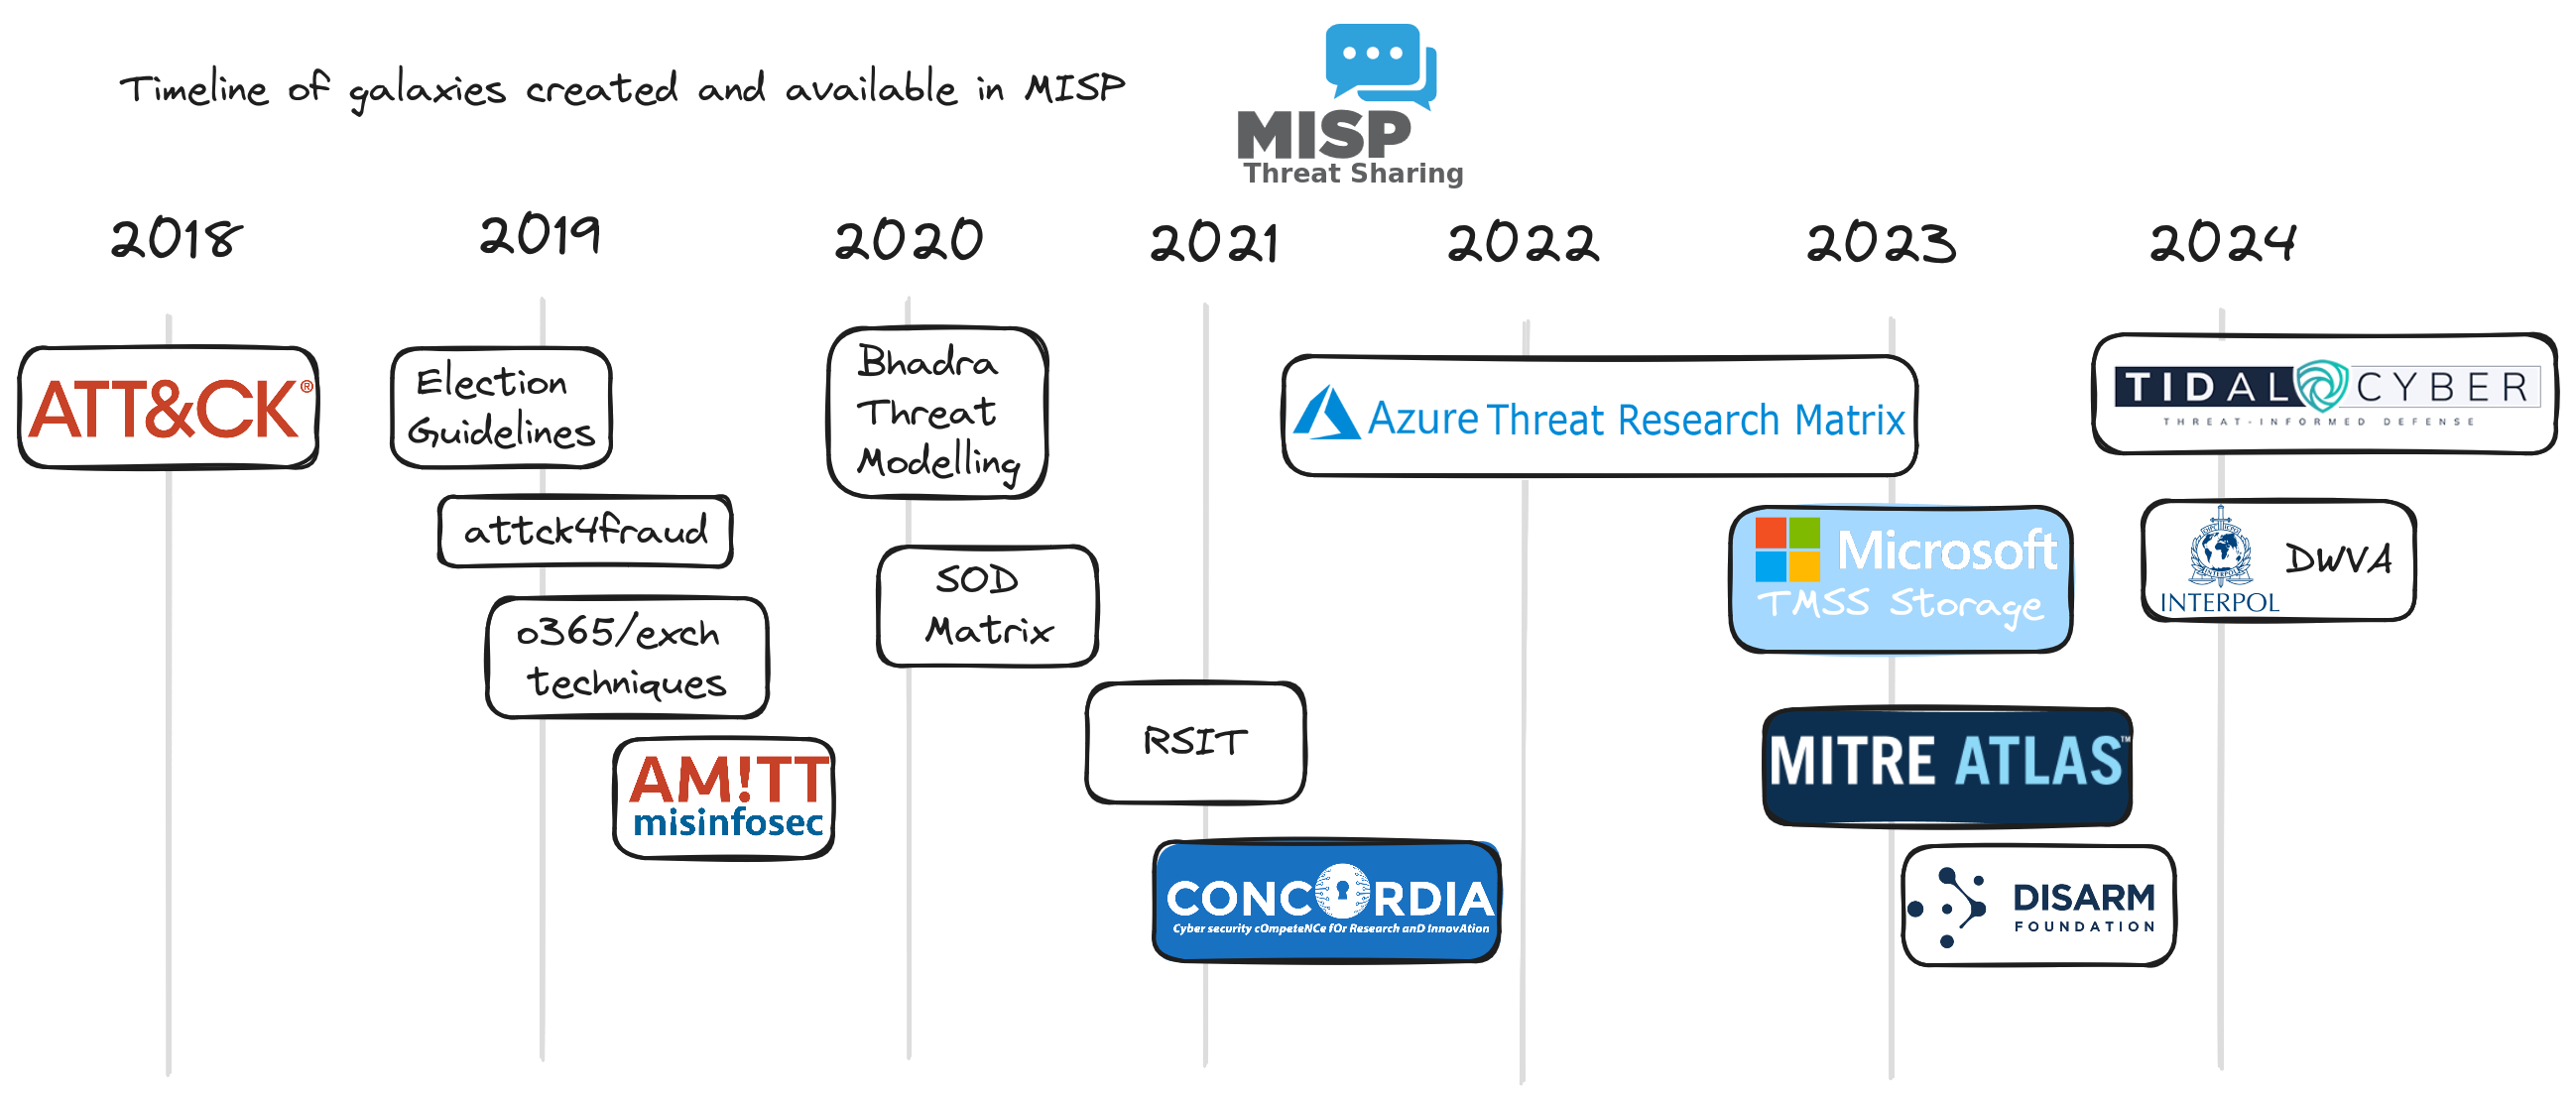
\includegraphics[scale=0.13]{./screenshots/timeline.png}
	\end{center}
\end{frame}

\begin{frame}
        \frametitle{What Leads to Starting New Frameworks?}
        \begin{itemize}
	\item New frameworks try to {\bf fill gaps}.
            \item New ideas in different areas/domains.
            \item Small vs. large initiatives.
	    \item {\bf Collaboration is not always easy}.
                \begin{itemize}
                    \item Small contributors vs. large organizations.
                    \item Absence of guidance to contribute.
                    \item Closed models.
                \end{itemize}
            \item Research \& publication vs. practical use.
            \item Need for timely new data in a continuously evolving threat landscape.
        \end{itemize}
\end{frame}

\begin{frame}
        \frametitle{Conversion (or the Dirty Part)}
        \begin{itemize}
            \item Understand the topic.
            \item Understand the users and their use cases.
            \item Map to Matrix / Kill Chain.
            \item Handle \textbf{various formats}:
                \begin{itemize}
                    \item JSON, XLS, PDF, DOCX, Markdown, CSV, web scraping, Python, etc.
                \end{itemize}
            \item Reverse engineer the data model.
            \item Manage UUIDs: existing vs. generating new.
            \item Handle duplicate values\footnote{In other words, many organizations didn’t machine-validate their own model.}:
                \begin{itemize}
                    \item Interaction with the framework owner.
                \end{itemize}
            \item Create the conversion script.
        \end{itemize}
\end{frame}


\begin{frame}
  \frametitle{Get in touch if you have any questions}
  \begin{itemize}
    \item MISP galaxy website \url{https://www.misp-galaxy.org/}
    \item Contact MISPProject 
    \begin{itemize}
      \item \url{https://github.com/MISP}
      \item \url{https://gitter.im/MISP/MISP}
      \item \url{https://twitter.com/MISPProject}
    \end{itemize}
  \end{itemize}
\end{frame}
